% TU Delft Beamer template
% Author: Maarten Abbink
% Delft University of Technology
% March 2014
% Version 2.0
% Based on original version 1.0 of Carl Schneider
\documentclass{beamer}
\usepackage{calc}
\usepackage[absolute,overlay]{textpos}
\usepackage[utf8]{inputenc}
\usepackage{polski}
\usepackage[polish]{babel}
\usepackage[document]{ragged2e}

\mode<presentation>{\usetheme{tud}}

\title[Metodyka PCM]{Przedstawienie metodyki PCM}
%\subtitle
\institute[ISI]{Inżynieria Systemów Informacyjnych}
\author{Anna Gawor, Dominik Pawlik}
\date{\today}

% Insert frame before each subsection (requires 2 latex runs)
\AtBeginSubsection[] {
	\begin{frame}<beamer>\frametitle{\titleSubsec}
		\tableofcontents[currentsection,currentsubsection]  % Generation of the Table of Contents
	\end{frame}
}
% Define the title of each inserted pre-subsection frame
\newcommand*\titleSubsec{Podrozdział}
% Define the title of the "Table of Contents" frame
\newcommand*\titleTOC{Zarys dokumentu}

% define a symbol which can be removed if you don't need it
\newcommand{\field}[1]{\mathbb{#1}}
\newcommand{\Zset}{\field{Z}}

\begin{document}

{
% remove the next line if you don't want a background image
\usebackgroundtemplate{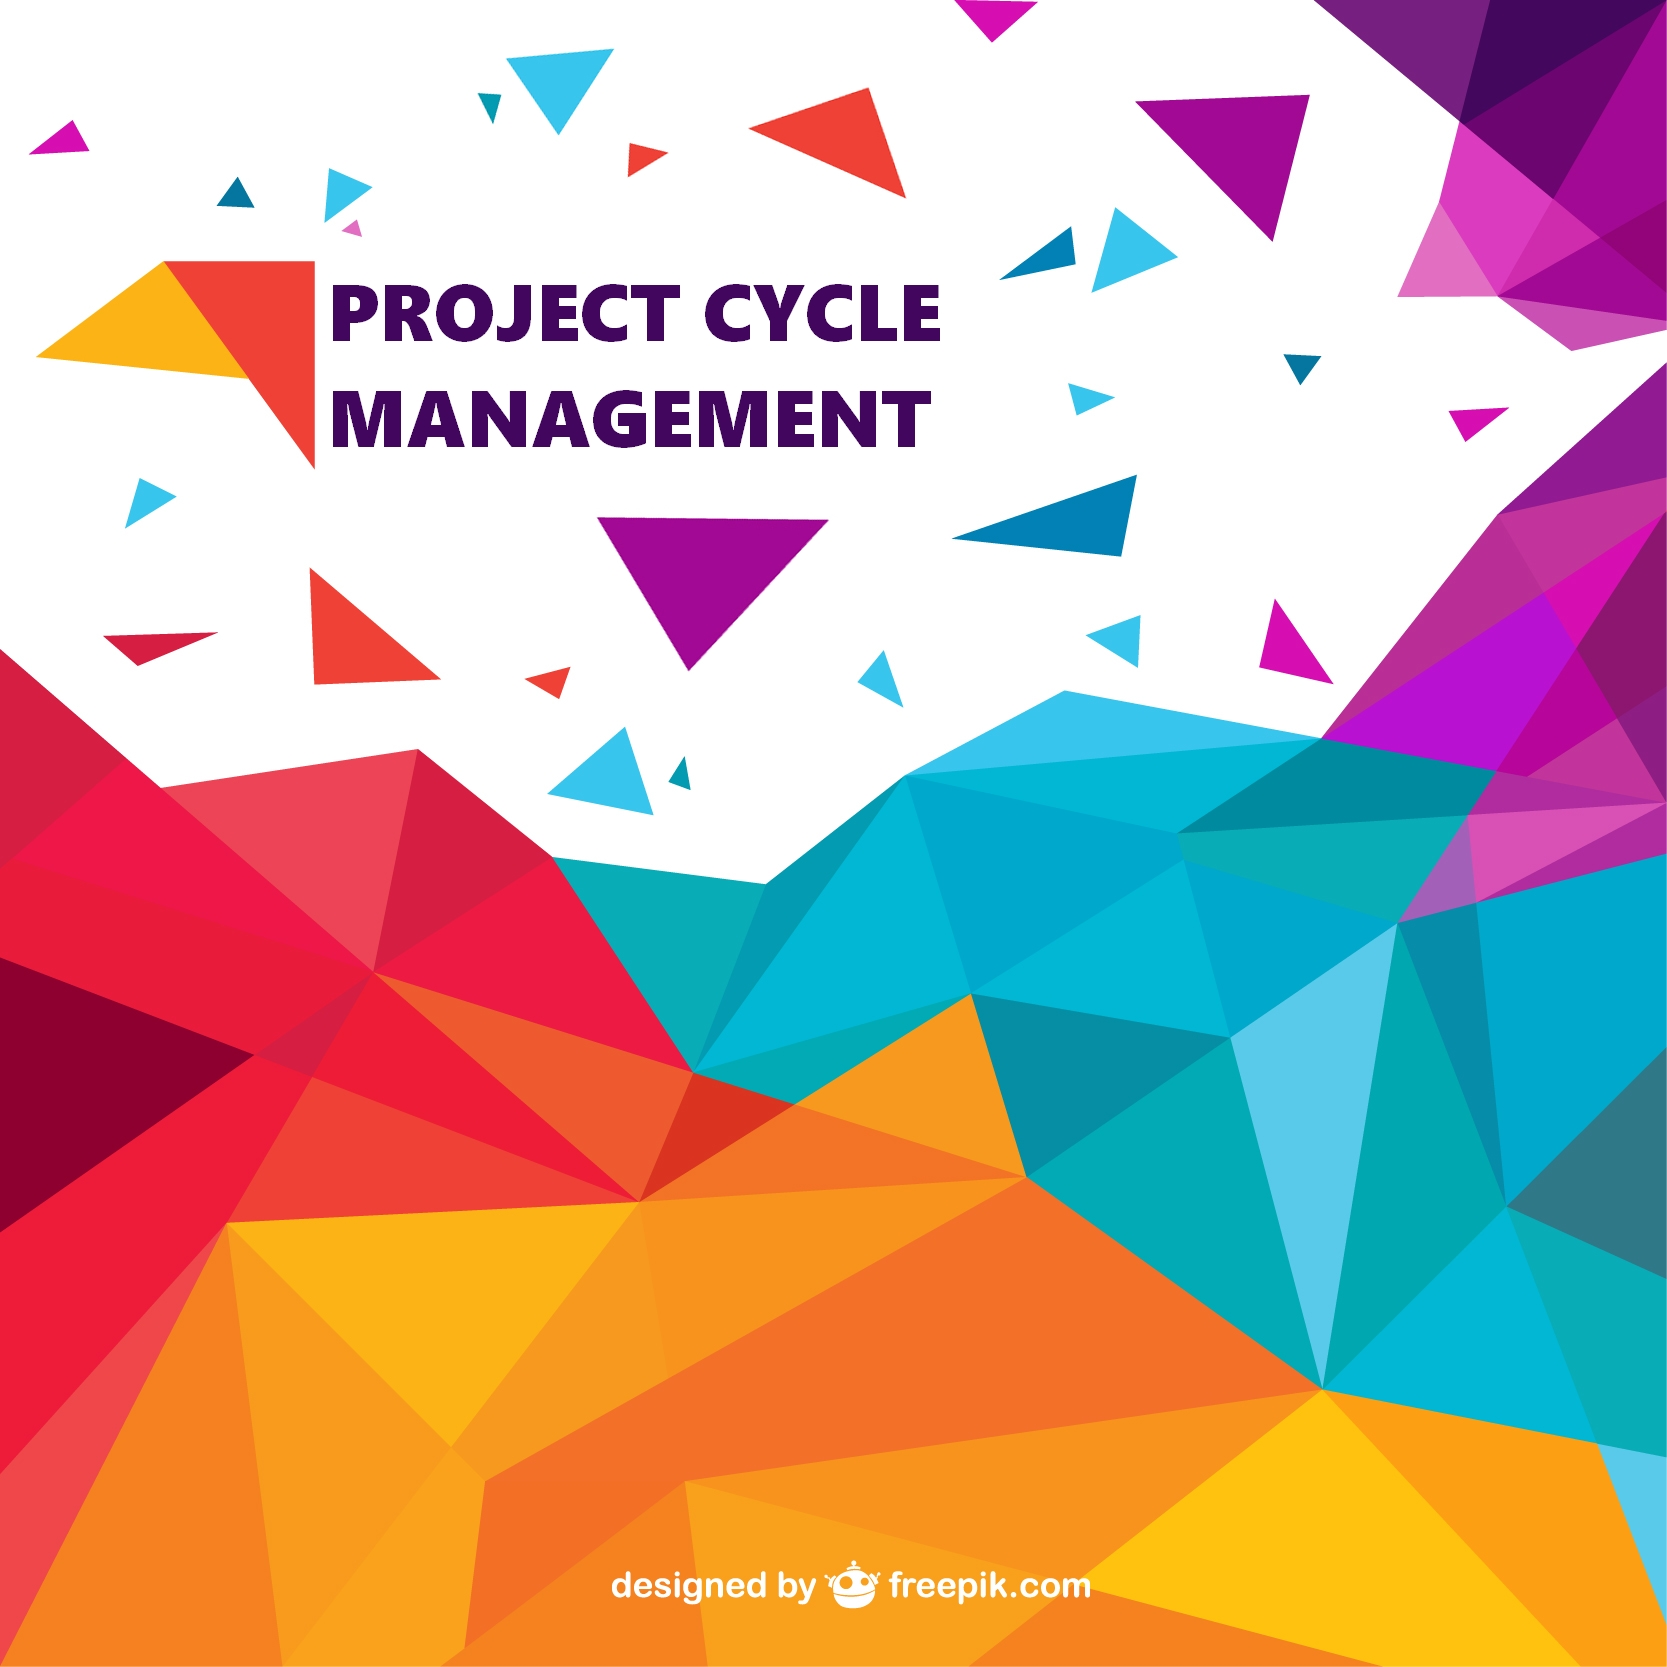
\includegraphics[width=\paperwidth,height=\paperheight]{images/tlo_latex.jpg}}%
\setbeamertemplate{footline}{\usebeamertemplate*{minimal footline}}
\frame{\titlepage}
}

{\setbeamertemplate{footline}{\usebeamertemplate*{minimal footline}}
\begin{frame}\frametitle{\titleTOC}
	\tableofcontents
\end{frame}
}

\section{Sekcja pierwsza}
\subsection{Wstęp do metodyki PCM}

\begin{frame}\frametitle{Wstęp do metodyki PCM}
    \begin{justify}
    Sposób, w jaki projekty są planowane oraz realizowane, przebiega według sekwencji określanej jako \textbf{cykl projektu}. Cykl życia projektu stanowi model realizacji projektu w czasie, określający zróżnicowanie sytuacji występujących w trakcie jego realizacji. Cykl rozpoczyna się od identyfikacji pomysłu i rozwija się w plan pracy, który może być wdrażany i oceniany. Pomysły są identyfikowane w kontekście uzgodnionej strategii.
    \textbf{PCM} gwarantuje, że projekty będą realizowane według określonej kolejności, wraz z oceną ich przydatności i wyjątkowości, co pozwala wyciągnąć wnioski dla przyszłych projektów. 
    \end{justify}
\end{frame}

\begin{frame}\frametitle{Wstęp do metodyki PCM}
	\begin{exampleblock}{PCM jest zestawem:}
        \begin{itemize}  
            \item koncepcji cyklu życia projektu,
            \item analizy interesariuszy
            \item narzędzi planowania (Macierz Logiczna),
            \item kluczowych czynników jakościowych,
            \item harmonogramów czynności i zasobów,
            \item standaryzowanych, spójnych struktur kluczowych dokumentów projektowych itd. \ldots 
        \end{itemize}
	%	\begin{minipage}{0.6\textwidth}
	%		% insert picture (pdf file)
	%		\includegraphics{images/ex1_periodic_number.pdf}
	%	\end{minipage}
	%	\centering{$u(n)=[3,1,4]_n$}
	    
	\end{exampleblock}
	Project Cycle Management (PCM) lub przekładając na język polski Zarządzanie Cyklem Projektu (ZCP) stanowi system zarządzania projektami. Powstał na potrzeby realizacji złożonych przedsięwzięć. 
\end{frame}

\begin{frame}\frametitle{Fazy PCM na wykresie}
	\begin{block}{Fazy PCM:}
		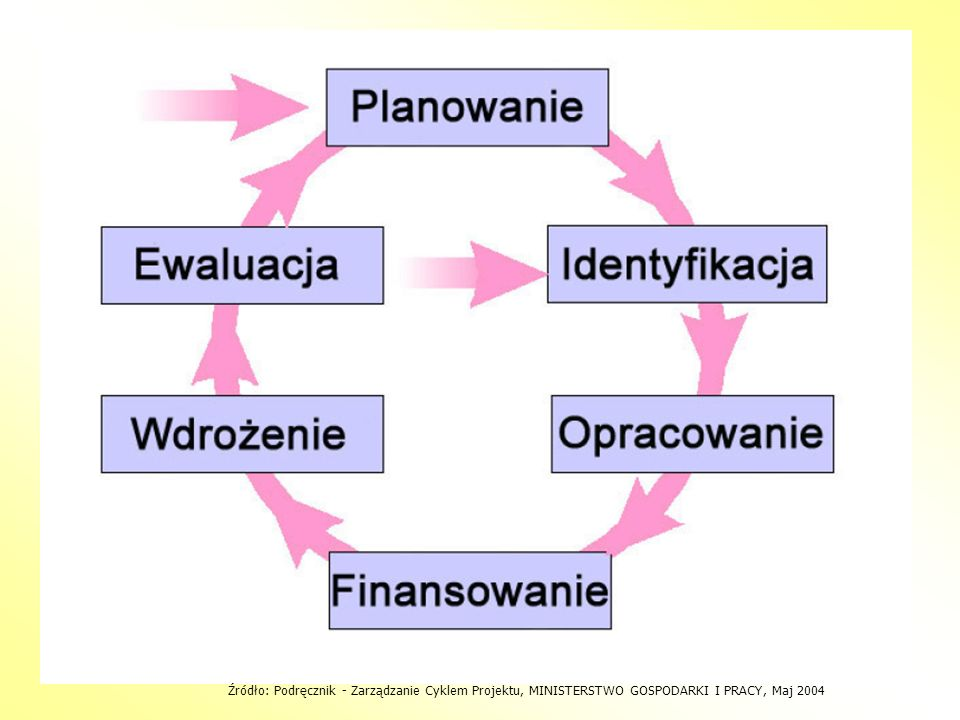
\includegraphics[scale=0.3]{images/fazy_latex.jpg}
		\centering
	\end{block}
\end{frame}

\begin{frame}\frametitle{Wytłumaczenie poszczególnych faz}
	\begin{exampleblock}{Fazy PCM:}
		\begin{itemize}
		    \item Planowanie - analiza sytuacji na poziomie narodowym i sektorowym tak, by określić problemy, ograniczenia i możliwości, które można by objąć projektem,
            \item Identyfikacja - sortowanie pomysłów na projekty do dalszej analizy, konsultacja z domyślnymi beneficjentami, określenia problemów, z którymi się stykają oraz sposobów ich rozwiązania,
            \item Opracowanie - wybrane pomysły projektów rozwijane są w operacyjne plany projektu. Następnie beneficjenci oraz interesariusze biorą udział w szczegółowym określeniu idei projektu. Następuje określenie wykonalności oraz trwałości,
	    \end{itemize}
	\end{exampleblock}
\end{frame}

\begin{frame}\frametitle{ }
	% Show first part of the screen highlighted
	\begin{exampleblock}{Fazy PCM:}
		\begin{itemize}
		    \item Finansowanie - następuje weryfikacja przez kompetentne władze i zapada decyzja o przekazaniu funduszy na projekt,
		    \item Wdrażanie - projekt jest uruchamiany i realizowany. W trakcie wdrażania kadra zarządzająca projektem ocenia aktualny postęp w stosunku do celów i dokonuje niezbędnych korekt,
		    \item Ewaluacja - instytucja finansująca projekt dokonuje oceny co zostało osiągnięte i co można poprawić w przyszłości.
		\end{itemize}
	\end{exampleblock}
\end{frame}

\subsection{Idea metodyki PCM}

\begin{frame}\frametitle{Idea metodyki PCM}
    \begin{columns}
    
		\column{0.60\textwidth}
        	\centering
        	
        	\begin{block}{Cele wprowadzenia PCM}
        	    \begin{itemize}
        	        \item słabe planowanie i przygotowanie projektów,
        	        \item projekty nieodpowiednie dla beneficjentów, 
        	        \item niewystarczające uwzględnianie zagrożeń, 
        	        \item ignorowanie czynników wpływających na trwałość korzyści projektów,
        	        \item nie wykorzystywanie doświadczeń wynikających z poprzednich projektów
        	    \end{itemize}
            \end{block}
        
		\column{0.4\textwidth}
    		\centering
    		
    		\begin{exampleblock}{Ciekawostka}
    	        \textbf{Zarządzanie Cyklem Projektu} zostało wprowadzone przez Komisję Europejską w początkach lat 90-tych w celu poprawy jakości tworzenia projektów i zarządzania, a w konsekwencji poprawy efektywności pomocy.
            \end{exampleblock}
			
	\end{columns}
	
\end{frame}


\subsection{Narzędzia zarządzania projektem}

\begin{frame}\frametitle{Narzędzia zarządzania projektami}
    \begin{columns}
    
		\column{0.40\textwidth}
        	\centering
        	
        	\begin{block}{LFA}
                \textbf{Logical Framework Approach} - narzędzie projektowania i zarządzania używanym w ramach PCM.
            \end{block}
        
		\column{0.6\textwidth}
    		\centering
    		
    		\begin{exampleblock}{Cel użycia}
    	        Zastosowanie tego narzędzia pozwala na identyfikację problemów oraz definiowanie działań prowadzących do rozwiązania problemów. Struktura ramy logicznej pozwala na weryfikację i przetestowanie modelu proponowanego projektu pod kątem jego trafności i wykonywalności.
            \end{exampleblock}
			
	\end{columns}
	
\end{frame}




\section{Podsumowanie}

\subsection{Gwarancje oferowane przez PCM}

\begin{frame}\frametitle{Gwarancje oferowane przez PCM cz.1}
    \begin{exampleblock}{PCM gwarantuje, że:}
    \begin{itemize}
        \item projekty odpowiadają uzgodnionej strategii oraz prawdziwym potrzebom beneficjentów: 
        \begin{itemize}
            \item projekty odpowiadają celom sektorowym, narodowym i europejskim, 
            beneficjenci są zaangażowani w proces planowania od wczesnego etapu,
            \item analiza problemu jest gruntowna, 
            \item cele są jasno formułowane w kategoriach korzyści dla grup docelowych; 
        \end{itemize}
        \item projekty są wykonalne pod względem realnych możliwości osiągnięcia celów: 
        \begin{itemize}
            \item cele są logiczne i mierzalne, 
            \item zagrożenia są brane pod uwagę, 
            \item monitorowanie koncentruje się na odpowiednich celach;
        \end{itemize}
    \end{itemize}

 


    \end{exampleblock}
\end{frame}

\begin{frame}\frametitle{Gwarancje oferowane przez PCM cz.2}
    \begin{exampleblock}{PCM gwarantuje, że:}
    \begin{itemize}
        \item projekty są trwałe: 
        \begin{itemize}
            \item czynniki wpływające na trwałość są uwzględniane w planie projektu,
            \item wyniki ewaluacji są wykorzystywane jako lekcja służąca do planowania przyszłych projektów.
        \end{itemize}
    \end{itemize}
    \end{exampleblock}
\end{frame}

\subsection[]{Podsumowanie}

\begin{frame}\frametitle{Podsumowanie}
	\begin{enumerate}
	    
	    \item Prawidłowa ocena prawdziwych potrzeb beneficjentów i wzięcie pod uwagę punktów widzenia różnych grup uczestników wymaga zebrania razem przedstawicieli wszystkich kluczowych uczestników w fazie analizy. W celu oszacowania czy plan projektu jest zgodny z różnymi rolami i potrzebami kobiet i mężczyzn niezbędne jest podejście oparte na płci.  

        \item Planowanie i realizowanie projektów przebiega według sekwencji, która określana jest jako cykl projektu. Tworzy on strukturę, która zapewnia konsultowanie wszystkich udziałowców, a także udostępnianie wszystkich informacji tak, by można było na tych informacjach oprzeć decyzje podejmowane w kluczowych fazach cyklu projektu. 
        
     
	\end{enumerate}
\end{frame}

\begin{frame}\frametitle{Podsumowanie}
	\begin{enumerate}
	    \setcounter{enumi}{2}
	   
        \item Rozdzielenie cyklu na sześć faz dostarcza minimalne podstawy dla efektywnego przygotowywania, wdrażania i ewaluacji projektu. Każda z faz prowadzi bezpośrednio do następnej. We wszystkich jednak, wymagane są informacje takie, by przed przejściem do następnej fazy podejmowane były rozsądne decyzje. Cykl oznacza, że wnioski wyciągnięte z zakończonych projektów pozwalają poprawić przyszłe projekty. 

        \item Oddzielenie fazy identyfikacji i opracowania jest szczególnie ważne. Poprzez dostosowanie do fazy identyfikacji, właściwość idei projektu może być ustalana systematycznie, zanim proces przygotowywania stanie się zbyt zaawansowany by można było porzucić określony pomysł. 

    \end{enumerate}
\end{frame}

\begin{frame}\frametitle{Podsumowanie}
	\begin{enumerate}
	   \setcounter{enumi}{4}
	   
        \item Stosowanie technik i narzędzi proponowanych w ramach ZCP zapewnia odpowiedniość projektów dla prawdziwych potrzeb beneficjentów, a także wykonalność i trwałość projektów. 

        \item Głównym rezultatem LFA jest matryca logiczna. Matryca logiczna wyznacza logikę interwencji projektu (jeśli działania są podejmowane wówczas osiągane będą rezultaty i zamierzenie projektu itd.) oraz opisuje ważne założenia i ryzyko kryjące się u podstawy logiki. Przy użyciu obiektywnie weryfikowalnych wskaźników i źródeł weryfikacji, matryca logiczna dostarcza szkieletu, według którego będzie monitorowany i oceniany postęp.


	\end{enumerate}
\end{frame}

\begin{frame}\frametitle{Literatura}

    \begin{thebibliography}{1}

          \bibitem{notes} http://www.up.gov.pl/efs/download/szkolenie\_PCM.pdf .
        
          \bibitem{impj}http://www.europeistyka.uj.edu.pl/documents/3458728/
          3814e0ac-4482-40b1-9247-410700011d39 .
        
          \bibitem{norman}http://www.frdl.org.pl/pliki/frdl/document/
          publikacjeFRDL\/PCM\_Zarzadzanie\_Cyklem\_Projektu.pdf .
        
          \bibitem{fo}"Podręcznik - Zarządzanie Cyklem Projektu"     MINISTERSTWO GOSPODARKI I PRACY, 2004 .

    \end{thebibliography}
         

\end{frame}

\end{document}
